\chapter{Matrizes}

\index{matriz}

Uma \key{matriz} é um conceito matemático
que corresponde a um array bidimensional
em programação. Por exemplo
\[
A = 
 \begin{bmatrix}
  6 & 13 & 7 & 4 \\
  7 & 0 & 8 & 2 \\
  9 & 5 & 4 & 18 \\
 \end{bmatrix}
\]
é uma matriz de tamanho $3 \times 4$, isto é,
ela possui 3 linhas e 4 colunas.
A notação $[i,j]$ refere-se
ao elemento na linha $i$ e coluna $j$
em uma matriz.
Por exemplo, na matriz acima,
$A[2,3]=8$ e $A[3,1]=9$.

\index{vetor}

Um caso especial de matriz é um \key{vetor},
que é uma matriz unidimensional de tamanho $n \times 1$.
Por exemplo,
\[
V =
\begin{bmatrix}
4 \\
7 \\
5 \\
\end{bmatrix}
\]
é um vetor que contém três elementos.

\index{transposta}

A \key{transposta} $A^T$ de uma matriz $A$
é obtida quando as linhas e colunas de $A$
são trocadas, ou seja, $A^T[i,j]=A[j,i]$:
\[
A^T = 
 \begin{bmatrix}
  6 & 7 & 9 \\
  13 & 0 & 5 \\
  7 & 8 & 4 \\
  4 & 2 & 18 \\
 \end{bmatrix}
\]

\index{matriz quadrada}

Uma matriz é uma \key{matriz quadrada} se ela
tiver o mesmo número de linhas e colunas.
Por exemplo, a seguinte matriz é uma
matriz quadrada:

\[
S = 
 \begin{bmatrix}
  3 & 12 & 4  \\
  5 & 9 & 15  \\
  0 & 2 & 4 \\
 \end{bmatrix}
\]

\section{Operações}

A soma $A+B$ das matrizes $A$ e $B$
é definida se as matrizes forem do mesmo tamanho.
O resultado é uma matriz onde cada elemento
é a soma dos elementos correspondentes
em $A$ e $B$.

Por exemplo,
\[
 \begin{bmatrix}
  6 & 1 & 4 \\
  3 & 9 & 2 \\
 \end{bmatrix}
+
 \begin{bmatrix}
  4 & 9 & 3 \\
  8 & 1 & 3 \\
 \end{bmatrix}
=
 \begin{bmatrix}
  6+4 & 1+9 & 4+3 \\
  3+8 & 9+1 & 2+3 \\
 \end{bmatrix}
=
 \begin{bmatrix}
  10 & 10 & 7 \\
  11 & 10 & 5 \\
 \end{bmatrix}.
\]

Multiplicar uma matriz $A$ por um valor $x$ significa
que cada elemento de $A$ é multiplicado por $x$.
Por exemplo,
\[
 2 \cdot \begin{bmatrix}
  6 & 1 & 4 \\
  3 & 9 & 2 \\
 \end{bmatrix}
=
 \begin{bmatrix}
  2 \cdot 6 & 2\cdot1 & 2\cdot4 \\
  2\cdot3 & 2\cdot9 & 2\cdot2 \\
 \end{bmatrix}
=
 \begin{bmatrix}
  12 & 2 & 8 \\
  6 & 18 & 4 \\
 \end{bmatrix}.
\]

\subsubsection{Multiplicação de Matrizes}

\index{multiplicação de matrizes}

O produto $AB$ das matrizes $A$ e $B$
é definido se $A$ for de tamanho $a \times n$
e $B$ for de tamanho $n \times b$, ou seja,
a largura de $A$ é igual à altura de $B$.
O resultado é uma matriz de tamanho $a \times b$
cujos elementos são calculados usando a fórmula
\[
AB[i,j] = \sum_{k=1}^n A[i,k] \cdot B[k,j].
\]

A ideia é que cada elemento de $AB$
é uma soma de produtos de elementos de $A$ e $B$,
de acordo com a seguinte figura:

\begin{center}
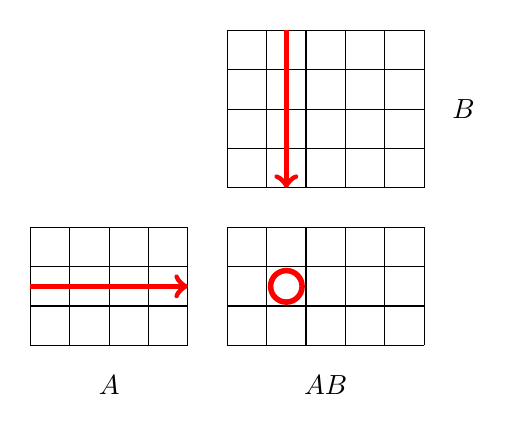
\begin{tikzpicture}[scale=0.5]
\draw (0,0) grid (4,3);
\draw (5,0) grid (10,3);
\draw (5,4) grid (10,8);

\node at (2,-1) {$A$};
\node at (7.5,-1) {$AB$};
\node at (11,6) {$B$};

\draw[thick,->,red,line width=2pt] (0,1.5) -- (4,1.5);
\draw[thick,->,red,line width=2pt] (6.5,8) -- (6.5,4);
\draw[thick,red,line width=2pt] (6.5,1.5) circle (0.4);
\end{tikzpicture}
\end{center}

Por exemplo,

\[
 \begin{bmatrix}
  1 & 4 \\
  3 & 9 \\
  8 & 6 \\
 \end{bmatrix}
\cdot
 \begin{bmatrix}
  1 & 6 \\
  2 & 9 \\
 \end{bmatrix}
=
 \begin{bmatrix}
  1 \cdot 1 + 4 \cdot 2 & 1 \cdot 6 + 4 \cdot 9 \\
  3 \cdot 1 + 9 \cdot 2 & 3 \cdot 6 + 9 \cdot 9 \\
  8 \cdot 1 + 6 \cdot 2 & 8 \cdot 6 + 6 \cdot 9 \\
 \end{bmatrix}
=
 \begin{bmatrix}
  9 & 42 \\
  21 & 99 \\
  20 & 102 \\
 \end{bmatrix}.
\]

A multiplicação de matrizes é associativa,
então $A(BC)=(AB)C$ é válido,
mas não é comutativa,
então $AB = BA$ geralmente não é válido.

\index{matriz identidade}

Uma \key{matriz identidade} é uma matriz quadrada
onde cada elemento na diagonal é 1
e todos os outros elementos são 0.
Por exemplo, a seguinte matriz
é a matriz identidade $3 \times 3$:
\[
 I = \begin{bmatrix}
  1 & 0 & 0 \\
  0 & 1 & 0 \\
  0 & 0 & 1 \\
 \end{bmatrix}
\]

\begin{samepage}
Multiplicar uma matriz por uma matriz identidade
não a altera. Por exemplo,
\[
 \begin{bmatrix}
  1 & 0 & 0 \\
  0 & 1 & 0 \\
  0 & 0 & 1 \\
 \end{bmatrix}
\cdot
 \begin{bmatrix}
  1 & 4 \\
  3 & 9 \\
  8 & 6 \\
 \end{bmatrix}
=
 \begin{bmatrix}
  1 & 4 \\
  3 & 9 \\
  8 & 6 \\
 \end{bmatrix} \hspace{10px} \textrm{e} \hspace{10px}
 \begin{bmatrix}
  1 & 4 \\
  3 & 9 \\
  8 & 6 \\
 \end{bmatrix}
\cdot
 \begin{bmatrix}
  1 & 0 \\
  0 & 1 \\
 \end{bmatrix}
=
 \begin{bmatrix}
  1 & 4 \\
  3 & 9 \\
  8 & 6 \\
 \end{bmatrix}.
\]
\end{samepage}

Usando um algoritmo padrão,
podemos calcular o produto de
duas matrizes $n \times n$
em tempo $O(n^3)$.
Existem também algoritmos mais eficientes
para multiplicação de matrizes\footnote{O primeiro algoritmo desse tipo
foi o algoritmo de Strassen,
publicado em 1969 \cite{str69},
cuja complexidade de tempo é $O(n^{2.80735})$;
o melhor algoritmo atual \cite{gal14}
funciona em tempo $O(n^{2.37286})$.},
mas eles são principalmente de interesse teórico,
e tais algoritmos não são necessários
em programação competitiva.


\subsubsection{Potência de Matrizes}

\index{potência de matrizes}

A potência $A^k$ de uma matriz $A$ é definida
se $A$ for uma matriz quadrada.
A definição é baseada na multiplicação de matrizes:
\[ A^k = \underbrace{A \cdot A \cdot A \cdots A}_{\textrm{$k$ vezes}} \]
Por exemplo,

\[
 \begin{bmatrix}
  2 & 5 \\
  1 & 4 \\
 \end{bmatrix}^3 =
 \begin{bmatrix}
  2 & 5 \\
  1 & 4 \\
 \end{bmatrix} \cdot
 \begin{bmatrix}
  2 & 5 \\
  1 & 4 \\
 \end{bmatrix} \cdot
 \begin{bmatrix}
  2 & 5 \\
  1 & 4 \\
 \end{bmatrix} =
 \begin{bmatrix}
  48 & 165 \\
  33 & 114 \\
 \end{bmatrix}.
\]
Além disso, $A^0$ é uma matriz identidade. Por exemplo,
\[
 \begin{bmatrix}
  2 & 5 \\
  1 & 4 \\
 \end{bmatrix}^0 =
 \begin{bmatrix}
  1 & 0 \\
  0 & 1 \\
 \end{bmatrix}.
\]

A matriz $A^k$ pode ser calculada eficientemente
em tempo $O(n^3 \log k)$ usando o
algoritmo do Capítulo 21.2. Por exemplo,
\[
 \begin{bmatrix}
  2 & 5 \\
  1 & 4 \\
 \end{bmatrix}^8 =
 \begin{bmatrix}
  2 & 5 \\
  1 & 4 \\
 \end{bmatrix}^4 \cdot
 \begin{bmatrix}
  2 & 5 \\
  1 & 4 \\
 \end{bmatrix}^4.
\]

\subsubsection{Determinante}

\index{determinante}

O \key{determinante} $\det(A)$ de uma matriz $A$
é definido se $A$ for uma matriz quadrada.
Se $A$ for de tamanho $1 \times 1$,
então $\det(A)=A[1,1]$.
O determinante de uma matriz maior é
calculado recursivamente usando a fórmula \index{cofator}
\[\det(A)=\sum_{j=1}^n A[1,j] C[1,j],\]
onde $C[i,j]$ é o \key{cofator} de $A$
em $[i,j]$.
O cofator é calculado usando a fórmula
\[C[i,j] = (-1)^{i+j} \det(M[i,j]),\]
onde $M[i,j]$ é obtido removendo
a linha $i$ e a coluna $j$ de $A$.
Devido ao coeficiente $(-1)^{i+j}$ no cofator,
cada determinante alterna entre positivo
e negativo.
Por exemplo,
\[
\det(
 \begin{bmatrix}
  3 & 4 \\
  1 & 6 \\
 \end{bmatrix}
) = 3 \cdot 6 - 4 \cdot 1 = 14 
\]
and
\[
\det(
 \begin{bmatrix}
  2 & 4 & 3 \\
  5 & 1 & 6 \\
  7 & 2 & 4 \\
 \end{bmatrix}
) = 
2 \cdot
\det(
 \begin{bmatrix}
  1 & 6 \\
  2 & 4 \\
 \end{bmatrix}
)
-4 \cdot
\det(
 \begin{bmatrix}
  5 & 6 \\
  7 & 4 \\
 \end{bmatrix}
)
+3 \cdot
\det(
 \begin{bmatrix}
  5 & 1 \\
  7 & 2 \\
 \end{bmatrix}
) = 81.
\]

\index{matriz inversa}

O determinante de $A$ nos diz
se existe uma \key{matriz inversa}
$A^{-1}$, tal que $A \cdot A^{-1} = I$,
onde $I$ é uma matriz identidade.
Acontece que $A^{-1}$ existe
exatamente quando $\det(A) \neq 0$,
e pode ser calculada usando a fórmula

\[A^{-1}[i,j] = \frac{C[j,i]}{det(A)}.\]

Por exemplo,

\[
\underbrace{
 \begin{bmatrix}
  2 & 4 & 3\\
  5 & 1 & 6\\
  7 & 2 & 4\\
 \end{bmatrix}
}_{A}
\cdot
\underbrace{
 \frac{1}{81}
 \begin{bmatrix}
   -8 & -10 & 21 \\
   22 & -13 & 3 \\
   3 & 24 & -18 \\
 \end{bmatrix}
}_{A^{-1}}
=
\underbrace{
 \begin{bmatrix}
  1 & 0 & 0 \\
  0 & 1 & 0 \\
  0 & 0 & 1 \\
 \end{bmatrix}
}_{I}.
\]

\section{Recorrências Lineares}

\index{recorrência linear}

Uma \key{recorrência linear}
é uma função $f(n)$
cujos valores iniciais são
$f(0),f(1),\ldots,f(k-1)$
e valores maiores
são calculados recursivamente usando a fórmula
\[f(n) = c_1 f(n-1) + c_2 f(n-2) + \ldots + c_k f (n-k),\]
onde $c_1,c_2,\ldots,c_k$ são coeficientes constantes.

A programação dinâmica pode ser usada para calcular
qualquer valor de $f(n)$ em tempo $O(kn)$, calculando
todos os valores de $f(0),f(1),\ldots,f(n)$ um após o outro.
No entanto, se $k$ for pequeno, é possível calcular
$f(n)$ de forma muito mais eficiente em tempo $O(k^3 \log n)$,
usando operações com matrizes.

\subsubsection{Números de Fibonacci}

\index{número de Fibonacci}

Um exemplo simples de uma recorrência linear é a
seguinte função que define os números de Fibonacci:
\[
\begin{array}{lcl}
f(0) & = & 0 \\
f(1) & = & 1 \\
f(n) & = & f(n-1)+f(n-2) \\
\end{array}
\]
Neste caso, $k=2$ and $c_1=c_2=1$.

\begin{samepage}
Para calcular números de Fibonacci de forma eficiente,
representamos a
fórmula de Fibonacci como uma
matriz quadrada $X$ de tamanho $2 \times 2$,
para a qual o seguinte é válido:
\[ X \cdot
 \begin{bmatrix}
  f(i) \\
  f(i+1) \\
 \end{bmatrix}
=
 \begin{bmatrix}
  f(i+1) \\
  f(i+2) \\
 \end{bmatrix}
 \]
Assim, os valores $f(i)$ e $f(i+1)$ são dados como
''entrada'' para $X$,
e $X$ calcula os valores $f(i+1)$ e $f(i+2)$
a partir deles.
Acontece que tal matriz é

\[ X = 
 \begin{bmatrix}
  0 & 1 \\
  1 & 1 \\
 \end{bmatrix}.
\]
\end{samepage}
\noindent
Por exemplo,
\[
 \begin{bmatrix}
  0 & 1 \\
  1 & 1 \\
 \end{bmatrix}
\cdot
 \begin{bmatrix}
  f(5) \\
  f(6) \\
 \end{bmatrix}
=
 \begin{bmatrix}
  0 & 1 \\
  1 & 1 \\
 \end{bmatrix}
\cdot
 \begin{bmatrix}
  5 \\
  8 \\
 \end{bmatrix}
=
 \begin{bmatrix}
  8 \\
  13 \\
 \end{bmatrix}
=
 \begin{bmatrix}
  f(6) \\
  f(7) \\
 \end{bmatrix}.
\]
Assim, podemos calcular $f(n)$ usando a fórmula
\[
 \begin{bmatrix}
  f(n) \\
  f(n+1) \\
 \end{bmatrix}
=
X^n \cdot
 \begin{bmatrix}
  f(0) \\
  f(1) \\
 \end{bmatrix}
=
 \begin{bmatrix}
  0 & 1 \\
  1 & 1 \\
 \end{bmatrix}^n
\cdot
 \begin{bmatrix}
  0 \\
  1 \\
 \end{bmatrix}.
\]
O valor de $X^n$ pode ser calculado em
tempo $O(\log n)$,
então o valor de $f(n)$ também pode ser calculado
em tempo $O(\log n)$.

\subsubsection{Caso Geral}

Agora, vamos considerar o caso geral em que
$f(n)$ é qualquer recorrência linear.
Novamente, nosso objetivo é construir uma matriz $X$
para a qual

\[ X \cdot
 \begin{bmatrix}
  f(i) \\
  f(i+1) \\
  \vdots \\
  f(i+k-1) \\
 \end{bmatrix}
=
 \begin{bmatrix}
  f(i+1) \\
  f(i+2) \\
  \vdots \\
  f(i+k) \\
 \end{bmatrix}.
\]
Tal matriz é
\[
X =
 \begin{bmatrix}
  0 & 1 & 0 & 0 & \cdots & 0 \\
  0 & 0 & 1 & 0 & \cdots & 0 \\
  0 & 0 & 0 & 1 & \cdots & 0 \\
  \vdots & \vdots & \vdots & \vdots & \ddots & \vdots \\
  0 & 0 & 0 & 0 & \cdots & 1 \\
  c_k & c_{k-1} & c_{k-2} & c_{k-3} & \cdots & c_1 \\
 \end{bmatrix}.
\]
Nas primeiras $k-1$ linhas, cada elemento é 0,
exceto que um elemento é 1.
Essas linhas substituem $f(i)$ por $f(i+1)$,
$f(i+1)$ por $f(i+2)$ e assim por diante.
A última linha contém os coeficientes da recorrência
para calcular o novo valor $f(i+k)$.

\begin{samepage}
Agora, $f(n)$ pode ser calculado em
tempo $O(k^3 \log n)$ usando a fórmula
\[
 \begin{bmatrix}
  f(n) \\
  f(n+1) \\
  \vdots \\
  f(n+k-1) \\
 \end{bmatrix}
=
X^n \cdot
 \begin{bmatrix}
  f(0) \\
  f(1) \\
  \vdots \\
  f(k-1) \\
 \end{bmatrix}.
\]
\end{samepage}

\section{Grafos e Matrizes}

\subsubsection{Contando Caminhos}

As potências de uma matriz de adjacência de um grafo
têm uma propriedade interessante.
Quando $V$ é uma matriz de adjacência de um grafo não ponderado,
a matriz $V^n$ contém os números de caminhos de
$n$ arestas entre os vértices no grafo.

Por exemplp, para o grafo
\begin{center}
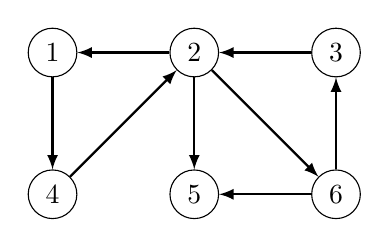
\begin{tikzpicture}[scale=0.9]
\node[draw, circle] (1) at (1,3) {$1$};
\node[draw, circle] (2) at (1,1) {$4$};
\node[draw, circle] (3) at (3,3) {$2$};
\node[draw, circle] (4) at (5,3) {$3$};
\node[draw, circle] (5) at (3,1) {$5$};
\node[draw, circle] (6) at (5,1) {$6$};

\path[draw,thick,->,>=latex] (1) -- (2);
\path[draw,thick,->,>=latex] (2) -- (3);
\path[draw,thick,->,>=latex] (3) -- (1);
\path[draw,thick,->,>=latex] (4) -- (3);
\path[draw,thick,->,>=latex] (3) -- (5);
\path[draw,thick,->,>=latex] (3) -- (6);
\path[draw,thick,->,>=latex] (6) -- (4);
\path[draw,thick,->,>=latex] (6) -- (5);
\end{tikzpicture}
\end{center}
a matriz de adjacência é
\[
V= \begin{bmatrix}
  0 & 0 & 0 & 1 & 0 & 0 \\
  1 & 0 & 0 & 0 & 1 & 1 \\
  0 & 1 & 0 & 0 & 0 & 0 \\
  0 & 1 & 0 & 0 & 0 & 0 \\
  0 & 0 & 0 & 0 & 0 & 0 \\
  0 & 0 & 1 & 0 & 1 & 0 \\
 \end{bmatrix}.
\]
Agora, por exemplo, a matriz
\[
V^4= \begin{bmatrix}
  0 & 0 & 1 & 1 & 1 & 0 \\
  2 & 0 & 0 & 0 & 2 & 2 \\
  0 & 2 & 0 & 0 & 0 & 0 \\
  0 & 2 & 0 & 0 & 0 & 0 \\
  0 & 0 & 0 & 0 & 0 & 0 \\
  0 & 0 & 1 & 1 & 1 & 0 \\
 \end{bmatrix}
\]
contém os números de caminhos de 4 arestas
entre os vértices.
Por exemplo, $V^4[2,5]=2$,
porque há dois caminhos de 4 arestas
do vértice 2 ao vértice 5:
$2 \rightarrow 1 \rightarrow 4 \rightarrow 2 \rightarrow 5$
e 
$2 \rightarrow 6 \rightarrow 3 \rightarrow 2 \rightarrow 5$.

\subsubsection{Caminhos mais Curtos}

Usando uma ideia semelhante em um grafo ponderado,
podemos calcular, para cada par de vértices, o comprimento mínimo de um caminho
entre eles que contém exatamente $n$ arestas.
Para calcular isso, temos que definir a multiplicação de matrizes
de uma nova maneira, para que não calculemos os números
de caminhos, mas minimizemos os comprimentos dos caminhos.

\begin{samepage}
Como exemplo, considere o seguinte grafo:
\begin{center}
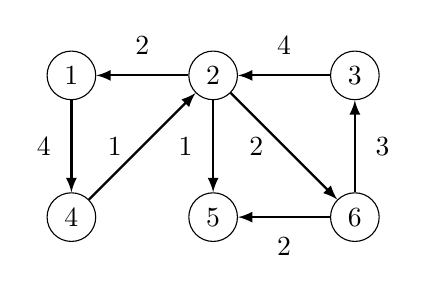
\begin{tikzpicture}[scale=0.9]
\node[draw, circle] (1) at (1,3) {$1$};
\node[draw, circle] (2) at (1,1) {$4$};
\node[draw, circle] (3) at (3,3) {$2$};
\node[draw, circle] (4) at (5,3) {$3$};
\node[draw, circle] (5) at (3,1) {$5$};
\node[draw, circle] (6) at (5,1) {$6$};

\path[draw,thick,->,>=latex] (1) -- node[font=\small,label=left:4] {} (2);
\path[draw,thick,->,>=latex] (2) -- node[font=\small,label=left:1] {} (3);
\path[draw,thick,->,>=latex] (3) -- node[font=\small,label=north:2] {} (1);
\path[draw,thick,->,>=latex] (4) -- node[font=\small,label=north:4] {} (3);
\path[draw,thick,->,>=latex] (3) -- node[font=\small,label=left:1] {} (5);
\path[draw,thick,->,>=latex] (3) -- node[font=\small,label=left:2] {} (6);
\path[draw,thick,->,>=latex] (6) -- node[font=\small,label=right:3] {} (4);
\path[draw,thick,->,>=latex] (6) -- node[font=\small,label=below:2] {} (5);
\end{tikzpicture}
\end{center}
\end{samepage}

Vamos construir uma matriz de adjacência onde
$\infty$ significa que uma aresta não existe,
e os outros valores correspondem aos pesos das arestas.
A matriz é
\[
V= \begin{bmatrix}
  \infty & \infty & \infty & 4 & \infty & \infty \\
  2 & \infty & \infty & \infty & 1 & 2 \\
  \infty & 4 & \infty & \infty & \infty & \infty \\
  \infty & 1 & \infty & \infty & \infty & \infty \\
  \infty & \infty & \infty & \infty & \infty & \infty \\
  \infty & \infty & 3 & \infty & 2 & \infty \\
 \end{bmatrix}.
\]

em vez da fórmula
\[
AB[i,j] = \sum_{k=1}^n A[i,k] \cdot B[k,j]
\]
agora usamos a fórmula
\[
AB[i,j] = \min_{k=1}^n A[i,k] + B[k,j]
\]
para multiplicação de matrizes, então calculamos
um mínimo em vez de uma soma
e uma soma de elementos em vez de um produto.
Após esta modificação,
as potências das matrizes correspondem
aos caminhos mais curtos no grafo.

Por exemplo, como
\[
V^4= \begin{bmatrix}
  \infty & \infty & 10 & 11 & 9 & \infty \\
  9 & \infty & \infty & \infty & 8 & 9 \\
  \infty & 11 & \infty & \infty & \infty & \infty \\
  \infty & 8 & \infty & \infty & \infty & \infty \\
  \infty & \infty & \infty & \infty & \infty & \infty \\
  \infty & \infty & 12 & 13 & 11 & \infty \\
 \end{bmatrix},
\]
podemos concluir que o comprimento mínimo de um caminho
de 4 arestas
do vértice 2 ao vértice 5 é 8.
Tal caminho é
$2 \rightarrow 1 \rightarrow 4 \rightarrow 2 \rightarrow 5$.

\subsubsection{Teorema de Kirchhoff}

\index{Teorema de Kirchhoff}
\index{árvore geradora}

O \key{Teorema de Kirchhoff}
%\footnote{G. R. Kirchhoff (1824--1887) foi um físico alemão.}
fornece uma maneira
de calcular o número de árvores geradoras
de um grafo como o determinante de uma matriz especial.
Por exemplo, o grafo
\begin{center}
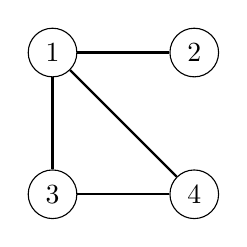
\begin{tikzpicture}[scale=0.9]
\node[draw, circle] (1) at (1,3) {$1$};
\node[draw, circle] (2) at (3,3) {$2$};
\node[draw, circle] (3) at (1,1) {$3$};
\node[draw, circle] (4) at (3,1) {$4$};

\path[draw,thick,-] (1) -- (2);
\path[draw,thick,-] (1) -- (3);
\path[draw,thick,-] (3) -- (4);
\path[draw,thick,-] (1) -- (4);
\end{tikzpicture}
\end{center}
possui três árvores geradoras:
\begin{center}
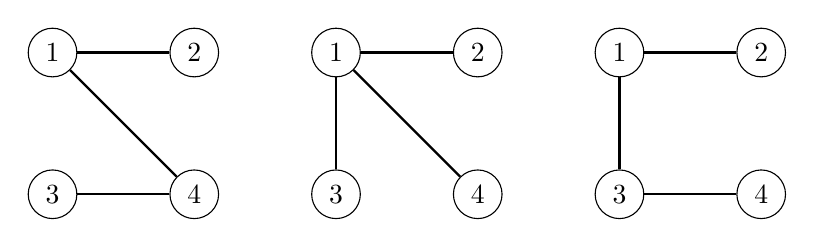
\begin{tikzpicture}[scale=0.9]
\node[draw, circle] (1a) at (1,3) {$1$};
\node[draw, circle] (2a) at (3,3) {$2$};
\node[draw, circle] (3a) at (1,1) {$3$};
\node[draw, circle] (4a) at (3,1) {$4$};

\path[draw,thick,-] (1a) -- (2a);
%\path[draw,thick,-] (1a) -- (3a);
\path[draw,thick,-] (3a) -- (4a);
\path[draw,thick,-] (1a) -- (4a);

\node[draw, circle] (1b) at (1+4,3) {$1$};
\node[draw, circle] (2b) at (3+4,3) {$2$};
\node[draw, circle] (3b) at (1+4,1) {$3$};
\node[draw, circle] (4b) at (3+4,1) {$4$};

\path[draw,thick,-] (1b) -- (2b);
\path[draw,thick,-] (1b) -- (3b);
%\path[draw,thick,-] (3b) -- (4b);
\path[draw,thick,-] (1b) -- (4b);

\node[draw, circle] (1c) at (1+8,3) {$1$};
\node[draw, circle] (2c) at (3+8,3) {$2$};
\node[draw, circle] (3c) at (1+8,1) {$3$};
\node[draw, circle] (4c) at (3+8,1) {$4$};

\path[draw,thick,-] (1c) -- (2c);
\path[draw,thick,-] (1c) -- (3c);
\path[draw,thick,-] (3c) -- (4c);
%\path[draw,thick,-] (1c) -- (4c);
\end{tikzpicture}
\end{center}
\index{matriz Laplaciana}
Para calcular o número de árvores geradoras,
construímos uma \key{matriz Laplaciana} $L$,
onde $L[i,i]$ é o grau do vértice $i$
e $L[i,j]=-1$ se houver uma aresta entre
os vértices $i$ e $j$ e, caso contrário, $L[i,j]=0$.
A matriz Laplaciana para o grafo acima é a seguinte:
\[
L= \begin{bmatrix}
  3 & -1 & -1 & -1 \\
  -1 & 1 & 0 & 0 \\
  -1 & 0 & 2 & -1 \\
  -1 & 0 & -1 & 2 \\
 \end{bmatrix}
\]

Pode-se mostrar que
o número de árvores geradoras é igual
ao determinante de uma matriz que é obtida
quando removemos qualquer linha e qualquer coluna de $L$.
Por exemplo, se removermos a primeira linha
e coluna, o resultado é

\[ \det(
\begin{bmatrix}
  1 & 0 & 0 \\
  0 & 2 & -1 \\
  0 & -1 & 2 \\
 \end{bmatrix}
) =3.\]
O determinante é sempre o mesmo,
independentemente de qual linha e coluna removemos de $L$.

Observe que a fórmula de Cayley no Capítulo 22.5 é
um caso especial do Teorema de Kirchhoff,
porque, em um grafo completo de $n$ vértices,

\[ \det(
\begin{bmatrix}
  n-1 & -1 & \cdots & -1 \\
  -1 & n-1 & \cdots & -1 \\
  \vdots & \vdots & \ddots & \vdots \\
  -1 & -1 & \cdots & n-1 \\
 \end{bmatrix}
) =n^{n-2}.\]



